\documentclass[twocolumn,floatfix,nofootinbib,aps]{revtex4-1}
\usepackage[utf8]{inputenc}

\usepackage{amsmath}    % need for subequations
\usepackage{amssymb}    % for symbols
\usepackage{graphicx}   % need for figures
\usepackage{verbatim}   % useful for program listings
\usepackage{color}      % use if color is used in text
\usepackage{subfigure}  % use for side-by-side figures
%\usepackage{hyperref}   % use for hypertext links, including those to external documents and URLs
\usepackage[capitalise]{cleveref}   % use for referencing figures/equations
\begin{document}

\title{Optimal Parameter Selection in Markov State Models for Biomolecular Conformational Dynamics}
\author{Robert T. McGibbon}
\author{Christian R. Schwantes}
\author{Vijay S. Pande}

\begin{abstract}
Likelihood framework for choosing the optimal number of states in a
Markov State Model
\end{abstract}

\maketitle

\section{Introduction}
Protein dynamics are an essential aspect of biomolecular function. These dynamics span a wide range of length scales, timescales and complexity, including folding and aggregation, the conformational change between functional native substates, ligand binding, and allostery. Whereas classical experimental probes have often been interpreted in two-state frameworks, ensemble measurements with increasingly high temporal resolution as well as sensitive single molecule probes have uncovered a vast array of complex kinetics occurring via various pathways and with multiple intermediates. But atomic-resolution structural characterization of these dynamics is often a Herculean challenge -- as molecular probes like F\"{o}rster resonance energy transfer, small-angle x-ray scattering, and nuclear magnetic resonance techniques measure complex projections of the intrinsic structural dynamics, generally reporting simultaneously on many degrees of freedom.

Computer simulations can complement experiments by providing atomic-resolution insight into the structural dynamics. With advances at the algorithmic, hardware, and software levels, modern molecular simulation paradigms, incorporating specialized or accelerated hardware, often in combination with highly parallel distributed computing frameworks, are capable of generating extensive simulation data sets. In fact, the minimally-biased kinetic analysis of such simulations is often a central bottleneck and presents a major challenge to the field. The analysis paradigms often entail the construction of lower resolution models parametrized from the high resolution simulation data set which capture the essential features in an interpretable framework. For example, by projecting the data down onto one or two degrees of freedom we create a simpler model for the system, such as one characterized by diffusion along a single reaction coordinate.

Markov state models (MSMs) are one approach for analyzing MD data sets and driving further MD simulations that are able to smoothly move between high and low-resolution models. Such detailed models maintain quantitative agreement with the underlying simulation data, while low-resolution models capture the salient features of the potential energy landscape, sacrificing some degree of model complexity. In an MSM, the dynamics are modeled as a memory-less jump process between a discrete set of conformational states. The two key quantities which define the MSM are thus the state definitions, an indicator function basis over phase space, and the pairwise transition probabilities or transition rates, which determine the kinetics.

A significant challenge in the automated construction of Markov state models is the choice of the number of states. Although classical Hamiltonian dynamics form a continuous-time Markov chain in $\mathbb{R}^{6N}$, the Markov property does not hold after the projecting the dynamics onto a basis of discrete indicator functions. In particular, when states contain within them free energy barriers of substantial magnitude, the validity of the Markov assumption begins to suffer considerably. While this source of modeling error can be addressed by increasing the number of microstates, the reduction in one error comes at the expense of the increase in another. This second source of error is statistical in origin. As the number of states in the model grows, so does the number of parameters required to completely specify the kinetic model between all pairs of states. Because the amount of data is constant, each additional parameter leads to a decrease in the amount of data available per model parameter, which makes the approach susceptible to over-fitting.

Here, we seek to build models that are \emph{suitably} complex, given the data, yielding complex descriptions of the system only to the extent that their additional parameters are implied by the observed dynamics. To that end, we introduce a new procedure for scoring the likelihood of an MSM, which, together with cross validation and the Bayesian information criterion (BIC), enables the optimal selection of the state space, which we express both in terms of the number of states and the clustering algorithm employed to group sampled conformations into states. This approach complements validation procedures performed primarily based on human intuition, such as Chapman-Kolmogorov tests, and enables the treatment of model selection as an optimization problem amenable to automated methods.

\section{Likelihood of a Markov State Model}
With the kinetic model expressed as a set of pairwise state to state transition probabilities at a given lag time, the likelihood of an ensemble of trajectories after projection into the indicator function basis is given simply by the product of the transition matrix elements along the observed trajectories. However, as we vary the number of states, it is not permissible to simply compare these likelihoods as part of an optimization of the state definitions. In doing so, the optimal model would always be the trivial one state model, whose computed likelihood is unity regardless of the data.

The appropriate likelihood is instead a path action in phase space, on which the discrete states are merely an indicator function basis. With $s(X)$ as the function mapping conformations into the indicator function basis set, $s : \mathbb{R}^{3N} \rightarrow \{1, 2, \ldots, K\}$, the likelihood can be written as

\begin{align}
P[x_{0...T-1}] dx^T = \prod_{i=0}^{T-1} T(s(x_i) \rightarrow s(x_{i+1})) \cdot \prod_{i=0}^{T} p_{s(x_i)}(x_{i})
\label{eq:like}
\end{align}

With a discrete, non-overlapping state space, the likelihood of a sampled trajectory can be decomposed into a product of terms of two types: the state to state transition probabilities, $T(s_i \rightarrow s_j)$, and so-called emission distributions of each state, the conditional probability of observing a conformation at a given location in phase space given that the conformation, $x_t$ is within a certain state, $s(x_t)$.

For example, consider two Markov state models sharing the same transition matrix, $T$. In one model, the state emission distributions are highly peaked at specific locations in phase space, whereas in the other model the emission distributions are uniform over the volume of the states. If an observed trajectory does go through the first models’ regions of high likelihood, it is appropriately termed a more likely model given the data.

However, models' long timescale behavior -- the rates and fluxes between metastable basins -- are independent of the choice of the emission distributions. The emission distributions characterize only the fine details of the equilibrium distribution within states, a quantity that the MSM approach does not seek to model; implicit in the decision to group conformations together into states is the idea that we decline to model the differences between conformations belonging to the same state. If such differences exist and are sufficiently large to warrant attention, than the states are too large.

Therefore, the most appropriate emission distribution for discrete state MSMs is that of the uniform distribution over the phase-space volume of the state. That is, the likelihood of observing a conformation in phase space given that the conformation is assigned to state $i$ is $0$ if the conformation is outside of the bounding volume of the state and constant if the conformation is within the volume. This constant is set so that the distribution integrates to $1$, and is thus the reciprocal volume of the microstate.

\begin{equation}
\label{eq:like_vol}
P[x_{0...T-1}] dx^T = \prod_{i=0}^{T-1} T(s(x_i) \rightarrow s(x_{i+1})) \cdot \prod_{i=0}^T \frac{1}{V_{s(x_{i})}}
\end{equation}

\section{Cross Validation and the Bayes Information Criterion}

\begin{figure}
\centering
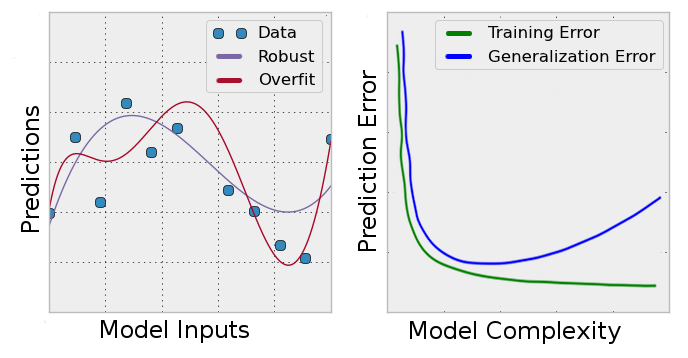
\includegraphics[width=3.1in]{figs/overfitting.png}
\caption{An example of overfitting. Left: in the presence of noise, a more complex model is able to fit the observed training data better, with lower residues and a higher empirical likelihood, but fails to distinguish the signal from the noise. Right: more complex model classes exhibit lower training errors, but generalize poorly to unobserved data.}
\end{figure}

Likelihood maximization is insufficient for model selection when the number of parameters varies between proposed models, as more complex models generally exhibit higher empirical likelihoods, often at the cost of larger generalization errors due to overfitting\cite{Hastie01Elements}. Statistical learning theory provides a number of alternative approaches for this problem. Conceptually, the most straightforward is a full Bayesian treatment in which all unknown model parameters are represented by probability distributions. The evidence for a model is computed by formally integrating over the model parameters and the evidence ratio, or Bayes factor\cite{Gelfand94Bayesian}, then provides a rigorous basis of model selection that appropriately punishes overly complex models as they become poorly constrained in parameter space. Unfortunately such approaches are intractable for problems of this size because of the need to integrate over all possible Markov models of a given size.

Instead, we explore both cross validation and Schwarz's Bayesian information criterion (BIC)\cite{Schwartz78Estimating} for choosing the number of states in a Markov state model. For cross validation, we parameterize the model, building both the state space and transition matrix on a subset of the data, but evaluating the likelihood on the left-out portion in an attempt to directly measure the generalization error. The BIC on the other hand involves augmenting the likelihood with a penalty on the number of parameters, and is
an asymptotic approximation Bayesian evidence.

\begin{equation}
\label{eq:bic}
\mathrm{BIC} \equiv -2\cdot \ln L + k \ln (n)
\end{equation}

where $L$ is the likelihood, $k$ is the number of free parameters, and $n$ is the number of data points, assumed to be independent and identically distributed.

\section{Computational Methods}

\begin{figure}
\centering
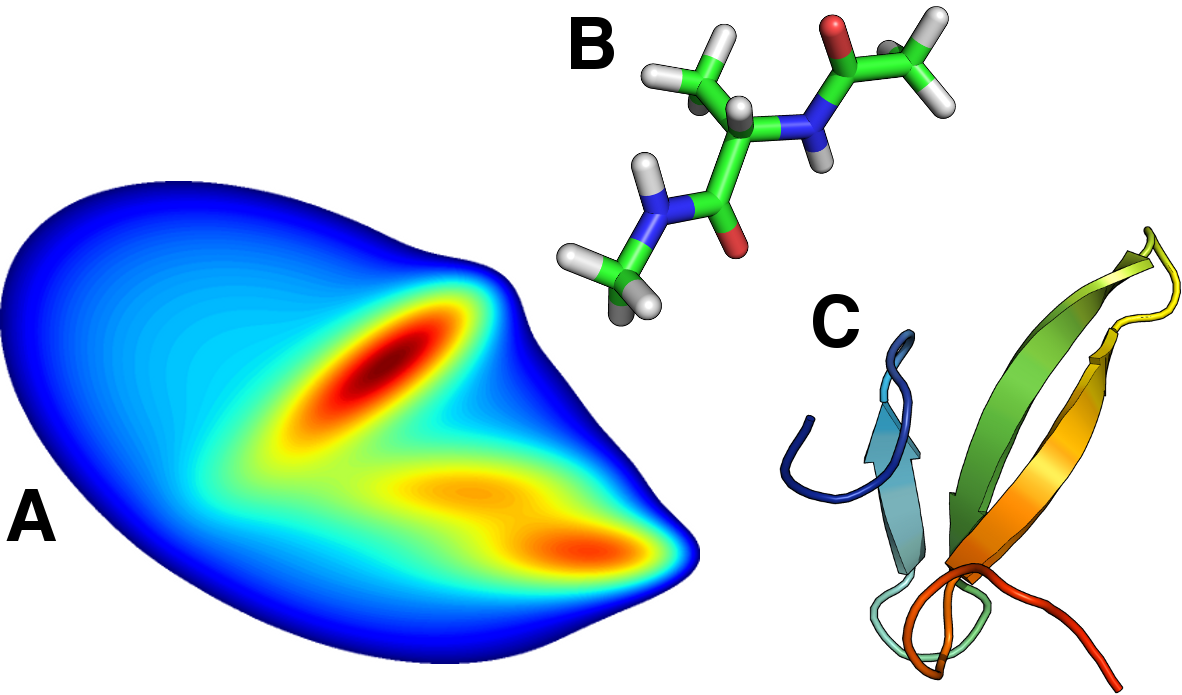
\includegraphics[width=3in]{figs/fig1_rbow.png}
\caption{Three systems studied in this work. (a) Langevin dynamics on the two dimensional M\"{u}ller potential. (b) 50 ns of dynamics of alanine dipeptide. (c) 200 $\mu s$ of dynamics of the Fip35 WW domain\cite{Liu2008Experimental}, courtesy of D.E. Shaw research \cite{}.}
\end{figure}

The uniform distribution emission model presents a computational challenge: its use requires the calculation of the (hyper)volume of the MSM's states, which, when defined by clustering are high-dimensional Voronoi cells. While trivial in two or three dimensions, this computational geometry task becomes challenging in high-dimensional settings. The computation of such volumes has occupied significant attention in recent years in the computational geometry literature, especially via randomized algorithms\cite{}. We opt to approximate the volumes using naive Monte Carlo rejection sampling, which we find tractable for large systems only when the molecular dynamics dataset is first projected into a suitable small vector space of up to perhaps ten dimensions.

A further challenge is the procedure by which to model the volume of states which are at the ``edge'' of the MSM -- whose Voronoi cells extend to infinity in some direction. Is the volume of these states unbounded? It is appropriate to assert that the volume of these edge states is bounded in some way by the extent of our dataset. For example, the volume of a state might be defined as the volume of the intersection of its Voronoi cell and the convex hull of the whole dataset, which would encode the assumption that the likelihood of observing conformations outside the convex hull of the sampled data is vanishing.

We use a slightly modified version of this definition that adopts the same spirit. Instead of taking the outer bounding envelope to be the convex hull of the data, we take it to be the set of all trial points such that the nearest sampled configuration to the trial point is closer than a certain cutoff, $R$. For further efficiency, it is feasible to use only a random subsample of the dataset for this nearest neighbor computation.

\section{Results and Discussion}
\subsection{M\"{u}ller Potential}
We simulated [HOW MANY STEPS?] of Langevin dynamics on the M\"{u}ller potential, clustered the data using the $k$-centers clustering algorithm with a euclidean distance metric, and computed the state volumes with [HOW MANY ROUNDS] of Monte carlo rejection sampling, using a padding distance of $R=?$ around the state centers from the 500 state model to define the datasets envelope.


\begin{figure}[h]
\centering
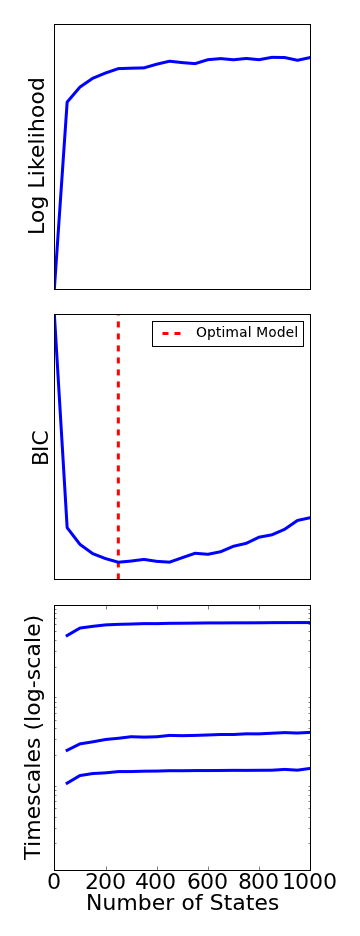
\includegraphics[width=2in]{figs/like_comp.png}
\caption{In models built using between 50 and 1,000 states with the $k$-centers algorithm, the log likelihood function increased quickly and plateaued at approximately 300 states, very close to the region in which the BIC is minimized. The BIC optimal model is also where the models' slowest implied timescals begins to become invariant with respect to the number of states.}
\label{fig:mullerlike}
\end{figure}

As shown in Fig. \ref{fig:mullerlike}, models built with too few states achieve a drastically reduced likelihood, but above a threshold region the likelihood increases relatively slowly. Here, the BIC's penalty on the number of parameters, which scales with the square of the number of states, begins to dominate. This model selection is consistent with tests based on the invariance of transition matrix eigenspectrum, but permits a direct optimization of the state space.

\begin{figure}
\centering
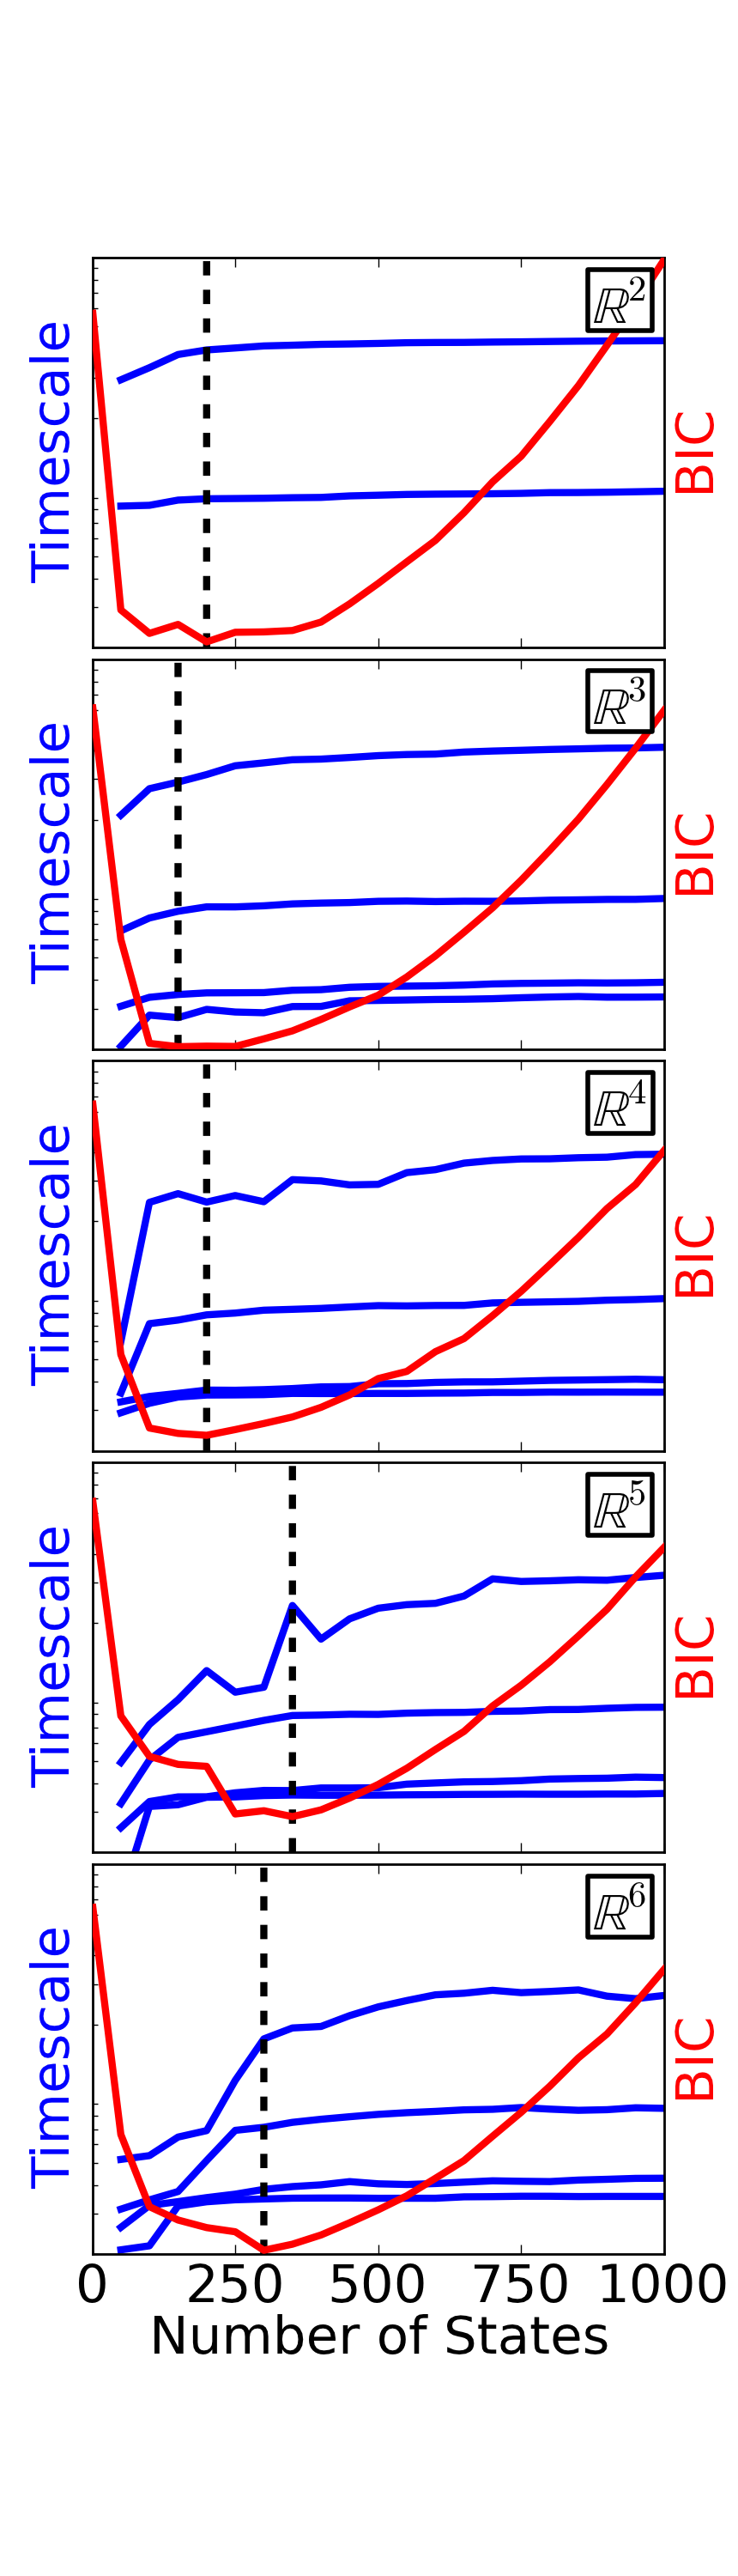
\includegraphics[width=2in]{figs/ww_bic_vs_eval_slide_nscounts.png}
\caption{Implied timescales and BIC scores for a series of Markov state models for the Fip35 WW domain. The panels differ by the dimensionality of the tICA projection. All models were built using Markovian lag time of [HOW MANY ns].}
\label{fig:ww}
\end{figure}

\subsection{Alanine Dipeptide}

\subsection{Fip35 WW Domain}

To test the procedure on a larger protein system, we reanalyzed two ultra-long 100 $\mu s$ molecular dynamics trajectories of the Fip35 WW domain\cite{Liu2008Experimental}, provided courtesy of D.E. Shaw Research \cite{}. In order to reduce the dimensionality of the problem, especially critical for the computation of the state volumes, we first preprocess the trajectories using time-structure based independent components analysis, retaining between two and six uncorrelated(?) linear combination of pairwise distances(?).

How many states are required for a Markov state model? Lane et. al., when analyzing this same dataset, proposed a 26,000 state Markov state model after clustering the data by RMSD, whereas Kellogg et. al. using an approach similar to that described herein, arrive at a [HOW MANY] state model after clustering on contact maps\cite{Lane2011Markov, Kellogg2012Evaluation}. 

\begin{itemize}
\item Is the 26,000 state model ``overfit''? The obvious answer, based on the line of reasoning that this paper is taking, is yes. But I think we need to consider the question a little more subtly. Perhaps it depends on what questions we ask of the model. When you ask both a ``properly-fit'' model and an overfit model a question that basically falls within the training set -- and neither of them need to extrapolate or really infer out-of-sample information, they'll both do fine. Heck, the overfit model might do better at telling you exactly what was \emph{in} the dataset.
\item The folding timescale is relatively insensitive to differences in MSM construction methodology. This has been observed in many datasets (McGibbon 2013, others). We hypothesize that this behavior is due to the large structural deviations at play -- even a two state model, given the same dataset, could basically get the right timescale just from counting the number of transitions. But finding these other timescales that are structurally subtle is different challenge. Also, how robust are other properties like experimental projections or the MFPT distribution to the number of states?
\item Single trajectory datasets are ``easier'' for MSMs. One of the uses of MSMs is to ``stich together'' multiple trajectories -- this function only happens when the states are large enough that they \emph{connect} trajectories, so you can't have too many states in this case. But when you have a single trajectory, there's no possible way to create a disconnected model anyways.
\item We need to state, elegantly if possible, the differences between our likelihood and Liz Kellogg's. This requires some careful language, since we think there are methodological problems with her approach.
\end{itemize}

\subsection{Limitations and Future Work}

\begin{itemize}
\item This model doesn't help us pick the lag time.
\item It also doesn't help us pick the projected vector space, at least in a quantitative way. This is kind of a big deal, but it is what it is.
\item Uniform distributions are extremely inconvenient to work with. In the future, we plan to extend this work to Markov state models without discrete states.
\item \{I want to get this in print.\} Going forward, we anticipate that a combination of kinetic dimensionality reduction and clustering is going to be the key combination for robust Markov state model construction. The two approaches are characterized by complementary approximations and sources of error. In dimensionality reduction, the assumption is that the dynamics ``align'' with the vectors in some sense -- we talk about dynamics in the ``x direction'' as having some characteristic, regardless of whether they occur around $x=x_a$ or $x=x_b$. In clustering, if $x_a$ and $x_b$ are in different states, there's no crosstalk at all. A euclidean distance metric is invariant with respect to unitary transforms anyways. But clustering gets ``thrown off'' when you have kinetically irrelevant directions: to get the same resolution with the clusters in the kinetically \emph{relevant} directions, you need a number of states that is exponential in the number of included kinetically \emph{irrelevant} directions. Because the sources of error are complementary, the combination should be uniquely powerful.
\end{itemize}


\section{Conclusions}
\begin{itemize}
    \item MSMs are great
    \item They have weaknesses. We are solving them.
    \item The automated selection of the number of states is a critical part of procedures that build MSMs as part of a simulation protocol to drive adaptive sampling. If MD algorithms required user input every couple picoseconds, people would never get anything done.
\end{itemize}

\bibliography{bibliography}
\end{document}
